%!TEX root = dsp_2nd_program_hw.tex
\subsection{DTMF Detection --- find\_dtmf\_symbol.h}
For convenience, we wrote a function to obtain the symbol of a DTMF signal.
By inputing the max two frequency, we can get the symbol $1,2,3,4,5,6,7,8,9,A,B,C,D,0,*,\#$

The code is shown in section~\ref{code:finddtmf}


\subsection{Recognition of Dataset 1 --- 10 signals}
	
\subsubsection{FFT --- DTMF\_1.cpp}
The result is 
$$5,1,6,9,8,7,3,4,0,2$$
for data
$$1081,1107,1140,1219,1234,1489,1507,1611,1942,1944$$
respectively, as shown in Table~\ref{tab:result}.
The code is shown in section~\ref{dtmf1}.

\begin{table}[htp]
\centering
{\small
\begin{tabular}{c|ccc}
    \hline
    \textbf{Signal length} & \textbf{1st freq} & \textbf{2nd freq} & \textbf{symbol} \\ 
    \hline
	   1081 & 769 & 1337 & 5 \\
	   1107 & 696 & 1212 & 1 \\
	   1140 & 770 & 1477 & 6 \\
	   1219 & 852 & 1477 & 9 \\
	   1234 & 852 & 1337 & 8 \\
	   1489 & 852 & 1212 & 7 \\
	   1507 & 696 & 1477 & 3 \\
	   1611 & 770 & 1212 & 4 \\
	   1942 & 942 & 1337 & 0 \\
	   1944 & 696 & 1337 & 2 \\
	\hline
\end{tabular}
}
\vspace{-0.1in}
\caption{DTMF result for 10 respective signals}
\label{tab:result}
\end{table}

\subsubsection{Goertzel --- DTMF\_2.cpp}
Goertzel has shown exactly same result with FFT. The code is shown in section~\ref{dtmf2}.








\newpage

\subsection{Recognition of Dataset 2 --- A long signal, DTMF\_3.cpp}

\subsubsection{Judge the start-end time}
By Matlab, we can obtain the time-zone signals as shown in Figure~\ref{fig:timezone3}. We then manually get the start, end time of each of signal as shown in Table~\ref{tab:startendtime}.
\begin{figure}[htp]
	\centering
	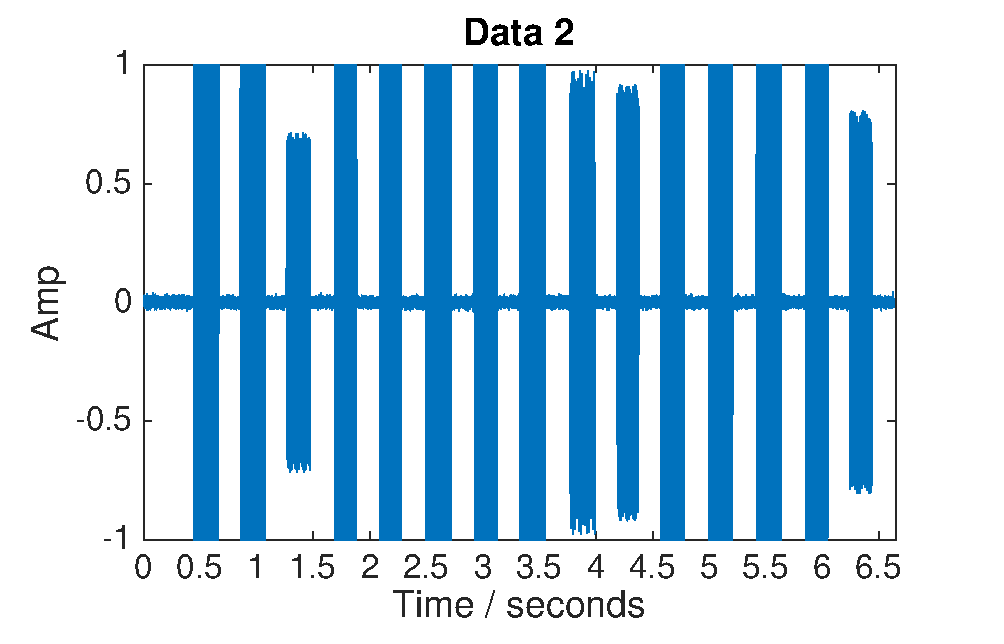
\includegraphics[width=10cm]{../fig/data2.eps}
	\vspace{-0.1in}
	\caption{Timezone signal of Data 2}
	\label{fig:timezone3}

\end{figure}
\vspace{-0.2in}

\begin{table}[htp]
\centering
{\small
\begin{tabular}{c|cc|c|cc}
    \hline
    \textbf{\#} & \textbf{Start time} & \textbf{End time} & \textbf{\#} & \textbf{Start time} & \textbf{End time} \\ 
    \hline
	   1 & 0.45 & 0.66	& 9   & 3.78 & 4.00	\\
	   2 & 0.86 & 1.07	& 10  & 4.18 & 4.40	\\
	   3 & 1.27 & 1.47	& 11  & 4.58 & 4.79	\\
	   4 & 1.70 & 1.89	& 12  & 5.01 & 5.22	\\
	   5 & 2.09 & 2.29	& 13  & 5.43 & 5.64	\\
	   6 & 2.50 & 2.72	& 14  & 5.87 & 6.06	\\
	   7 & 2.92 & 3.10	& 15  & 6.26 & 6.45	\\
	   8 & 3.34 & 3.55	& & &\\
	\hline
\end{tabular}
}
\vspace{-0.1in}
\caption{Start-End time of each signal}
\label{tab:startendtime}
\end{table}
\vspace{-0.3in}

\subsubsection{Result}
By the Goertzel method, we can obtain the symbols for the long signal are:
$$2,0,5,8,9,1,1,3,2,0,u,4,6,4,9$$
$u$ represents unknown, i.e. we cannot detect the 11th symbol, its amplitude response is shown in Figure~\ref{fig:freq11}.From the figure, we can see that we don't have two target frequencies which have a significant amplitude, s.t. we cannot decipher this symbol. The code is shown in section~\ref{dtmf3}.
\begin{figure}[htp]
	\centering
	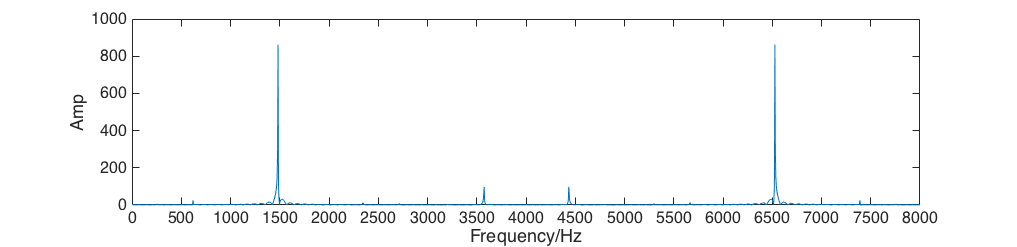
\includegraphics[width=16cm]{../fig/freq_11.png}
	\caption{Amplitude response of the 11th symbol}
	\label{fig:freq11}
\end{figure}





